\begin{activity} \label{A:3.2.2} 
 Consider the two-parameter family of functions of the form $h(x) = a(1-e^{-bx}),$ where $a$ and $b$ are positive real numbers.
	 \ba
		\item Find the first derivative and the critical values of $h$.  Use these to construct a first derivative sign chart and determine for which values of $x$ the function $h$ is increasing and decreasing. 
	 	\item Find the second derivative and build a second derivative sign chart.  For which values of $x$ is a function in this family concave up?  concave down?
		\item What is the value of $\ds \lim_{x \to \infty} a(1-e^{-bx})$? $\ds \lim_{x \to -\infty} a(1-e^{-bx})$?
		\item How does changing the value of $b$ affect the shape of the curve?
	  	\item Without using a graphing utility, sketch the graph of a typical member of this family. Write several sentences to describe the overall behavior of a typical function $h$ and how this behavior depends on $a$ and $b$.
	 \ea
\end{activity}
\begin{smallhint}
	 \ba
		\item Expand to write $h(x) = a - ae^{-bx}$ before differentiating.
	 	\item Remember that $e^{-bx}$ is never zero and always positive, regardless of the value of $x$.
		\item Recall that $e^{-x} \to 0$ as $x \to \infty$ and $e^{-x} \to \infty$ as $x \to -\infty$.
		\item Consider how $b$ affects the value of $h'(x)$.
	  	\item Use your work in (a)-(d).
	 \ea
\end{smallhint}
\begin{bighint}
	 \ba
		\item Expand to write $h(x) = a - ae^{-bx}$ before differentiating, and remember to treat $a$ and $b$ as constants.
	 	\item Remember that $e^{-bx}$ is never zero and always positive, regardless of the value of $x$, and that $a$ and $b$ are positive constants.
		\item Recall that $e^{-x} \to 0$ as $x \to \infty$ and $e^{-x} \to \infty$ as $x \to -\infty$.
		\item Consider how $b$ affects the value of $h'(x)$.
	  	\item Use your work in (a)-(d).
	 \ea
\end{bighint}
\begin{activitySolution}
\ba
  \item Since $h(x) = a - ae^{-bx}$, we have by the constant multiple and chain rules that
  $$h'(x) = -ae^{-bx}(-b) = abe^{-bx}.$$
  Since $a$ and $b$ are positive constants and $e^{-bx} > 0$ for all $x$, we see that $h'(x)$ is never zero (nor undefined), and indeed $h'(x) > 0$ for all $x$.  Hence $h$ is an always increasing function.
  \item Because $h'(x) = abe^{-bx},$ we have that $h''(x) = abe^{-bx}(-b) = -ab^2e^{-bx}$.  As with $h'$, we recognize that $a$, $b^2$, and $e^{-bx}$ are always positive, and thus $h''(x) = -ab^2e^{-bx} < 0$ for all values of $x$, making $h$ always concave down.
  \item As $x \to \infty$, $e^{-bx} \to 0$.  Thus,
  $$\lim_{x \to \infty} a(1-e^{-bx}) = \lim_{x \to \infty} a - ae^{-bx} = a - 0 = a.$$
  This shows that $h$ has a horizontal asymptote at $y = a$ as we move rightward on its graph.
  
  As $x \to -\infty$, $e^{-bx} \to \infty$.  Thus, 
  $$\lim_{x \to \infty} a(1-e^{-bx}) = \lim_{x \to \infty} a - ae^{-bx} = -\infty.$$
  \item Noting that $h'(x) = abe^{-bx}$, we see that if we consider different values of $b$, the slope of the graph changes.  If $b$ is large and $x$ is close to zero, $h'(x) \approx ab$ (since $e^0 = 1$), so $h'(x)$ is relatively large near $x = 0$.  At the same time, for large $b$, $e^{-bx}$ approaches zero quickly as $x$ increases, so the curve's slope will quickly approach zero as $x$ increases.  If $b$ is small, the graph is less steep near $x = 0$ and its slope goes to zero less quickly as $x$ increases.
  \item Observing that $h(0) = 0$ and $\lim_{x \to \infty} h(x) = a$, along with the facts that $h$ is always increasing and always concave down, we see that a typical member of this family looks like the following graph.
    \begin{center}
  	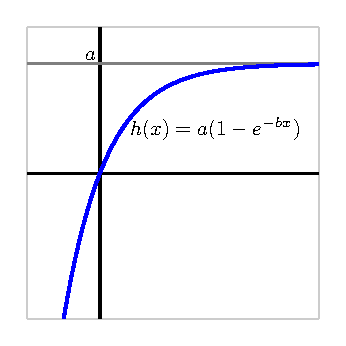
\includegraphics{figures/3_2_Act2Soln.eps}
  \end{center}	
\ea
\end{activitySolution}
\aftera